\documentclass{../template/Report}%方括号内写yuxi即生成预习报告\documentclass[yuxi]{../template/Report}
\settemplatedir{../template/}%设置模板路径

\exname{} %实验名称
\extable{} %实验桌号
\instructor{} %指导教师
\class{} %班级
\name{} %姓名
\stuid{} %学号

\nyear{} %年
\nmonth{} %月
\nday{} %日
\nweekday{} %星期几，e.g. \nweekday{三}
\daypart{}%上午/下午

\redate{} %如有实验补做，补做日期
\resitu{} %情况说明：

\begin{document}
\maketitle%输出封面

\section{预习报告（10分）}
\subsection{实验综述（5分）}
\subsubsection{实验原理}
\begin{enumerate}
    \item \textbf{内阻测定（替代法）}：利用电阻箱模拟表头在电路中的阻碍作用。如图\ref{fig:circuits}(a)，当电阻箱接入电路后的电流与接入表头时的电流（$I_0$）一致时，认为电阻箱阻值等于表头内阻 $R_g$。
    \item \textbf{量程扩展原理}：
          \begin{itemize}
              \item \textbf{电流表}：根据并联分流原理，在表头两端并联电阻 $R_1$（图b），分担 $I_1 - I_g$ 的电流。
              \item \textbf{电压表}：根据串联分压原理，在表头（或改装电流表）上串联电阻 $R_3$（图c），承担 $U_1 - U_g'$ 的电压。
          \end{itemize}
    \item \textbf{欧姆表原理}：基于闭合电路欧姆定律（图d）。电源电动势 $\varepsilon$ 恒定时，回路电流 $I$ 随外接电阻 $R_x$ 变化，即 $I = \frac{\varepsilon}{R_{\text{内}} + R_x}$，通过电流刻度标示电阻值。
\end{enumerate}

\subsubsection{实验流程}
\begin{enumerate}
    \item \textbf{测定内阻}：搭建替代法电路，精确测定微安表内阻 $R_g$。
    \item \textbf{改装与校准电流表}：
          \begin{itemize}
              \item 计算分流电阻 $R_1 = \frac{I_g R_g}{I_1 - I_g}$，调节电阻箱并接入。
              \item 与标准表比对，若读数偏小（分流过大），则需\textbf{增大} $R_1$，反之减小，直至误差合规。
          \end{itemize}
    \item \textbf{改装与校准电压表}：
          \begin{itemize}
              \item 计算分压电阻 $R_3 = \frac{U_1}{I_1} - R_{\text{表}}$，调节电阻箱并串联接入。
              \item 与标准表比对，若读数偏小（分压过大），则需\textbf{减小} $R_3$，反之增大。
          \end{itemize}
    \item \textbf{组装欧姆表}：连接电路，短接调零后，测量电阻箱不同阻值下的电流值，绘制刻度曲线。
\end{enumerate}

\begin{figure}[H]
    \centering
    \begin{subfigure}[b]{0.23\textwidth}
        
\includegraphics[width=\textwidth]{tidaifa.png}
        \caption{内阻测定}
    \end{subfigure}
    \hfill
    \begin{subfigure}[b]{0.23\textwidth}
        
\includegraphics[width=\textwidth]{gaizhuangA.png}
        \caption{改电流表}
    \end{subfigure}
    \hfill
    \begin{subfigure}[b]{0.23\textwidth}
        
\includegraphics[width=\textwidth]{gaizhuangV.png}
        \caption{改电压表}
    \end{subfigure}
    \hfill
    \begin{subfigure}[b]{0.23\textwidth}
        
\includegraphics[width=\textwidth]{gaizhuangOhm.png}
        \caption{改欧姆表}
    \end{subfigure}
    \caption{实验原理与改装电路图}
    \label{fig:circuits}
\end{figure}

\subsection{实验重点（3分）}
\begin{enumerate}
    \item 掌握替代法测量微安表内阻的操作细节。
    \item 熟练运用分流与分压公式计算电阻箱阻值，实现量程扩展。
    \item 掌握改装表的校准方法，特别是根据测量误差（偏大或偏小）反向推导并调整电阻箱阻值的策略。
\end{enumerate}

\subsection{实验难点（2分）}
\begin{enumerate}
    \item 校准过程中的逻辑判断：当改装表读数与标准表不符时，需准确判断是增大还是减小电路中的电阻箱阻值。
    \item 正确计算并调整电阻箱组织：需根据实际测量数据反复计算，确保分流或分压电阻阻值的准确性。
    \item 实验操作繁琐：涉及多次电路拆装与重组，接线较多，容易出现接触不良或接线错误导致的系统误差。
\end{enumerate}
\begin{fullreportonly}
    \section{原始数据（20分）}
    （将有老师签名的“自备数据记录草稿纸”的扫描或手机拍摄图粘贴在下方，完整保留姓名，学号，教师签字和日期。）

    \section{结果与分析}
    \subsection{数据处理与结果}

    \subsubsection{预备实验}
    本实验采用替代法和中值法对微安表头参数进行测定，测得表头内阻为 $R_g = \SI{232}{\ohm}$。

    \subsubsection{毫安表的设计、改装与校准}
    改装后的电流表量程为 $\SI{5}{\milli A}$，分度值为 $\SI{0.1}{\milli A}$。
    校准实验数据记录于 \cref{tableA} 中。其中示值误差 $\Delta I = I_{\text{标准}} - I_{\text{改装}}$。

    \begin{table}[H]
        \centering
        \caption{改装 $\SI{5}{\milli A}$ 电流表校准数据记录}
        \begin{tabular}{C{0.1\textwidth} C{0.15\textwidth} C{0.15\textwidth} C{0.15\textwidth} C{0.15\textwidth} C{0.15\textwidth}}
            \toprule
            序号 & $I_{\text{G}} (\si{mA})$ & $I_{\text{B}} (\si{mA})$ & $\Delta I (\si{mA})$ & $\varepsilon_r$ & $R_2 (\si{\ohm})$ \\
            \midrule
            1  & 1.00                     & 0.95                     & -0.05                & -5.3\%          & 57.0              \\
            2  & 2.00                     & 2.00                     & 0.00                 & 0.0\%           & 57.0              \\
            3  & 3.00                     & 3.02                     & 0.02                 & 0.7\%           & 57.0              \\
            4  & 4.00                     & 4.00                     & 0.00                 & 0.0\%           & 57.0              \\
            5  & 5.00                     & 5.00                     & 0.00                 & 0.0\%           & 57.0              \\
            \bottomrule
        \end{tabular}
        \label{tableA}
    \end{table}

    计算得最大绝对误差 $\Delta_{max} = |-0.05| = \SI{0.05}{\milli A}$。
    根据准确度等级判定指数 $\alpha = \left| \frac{\Delta_{max}}{0.1} \right| = \left| \frac{0.05}{0.1} \right| = 0.5$，故该改装电流表的准确度等级定为 0.5 级。
    改装表读数 $I_G$ 与标准值 $I_B$ 的对应关系及误差分布如 \cref{fig:ampere_analysis} 所示。

    \begin{figure}[H]
        \centering
        \begin{subfigure}[b]{0.48\textwidth}
            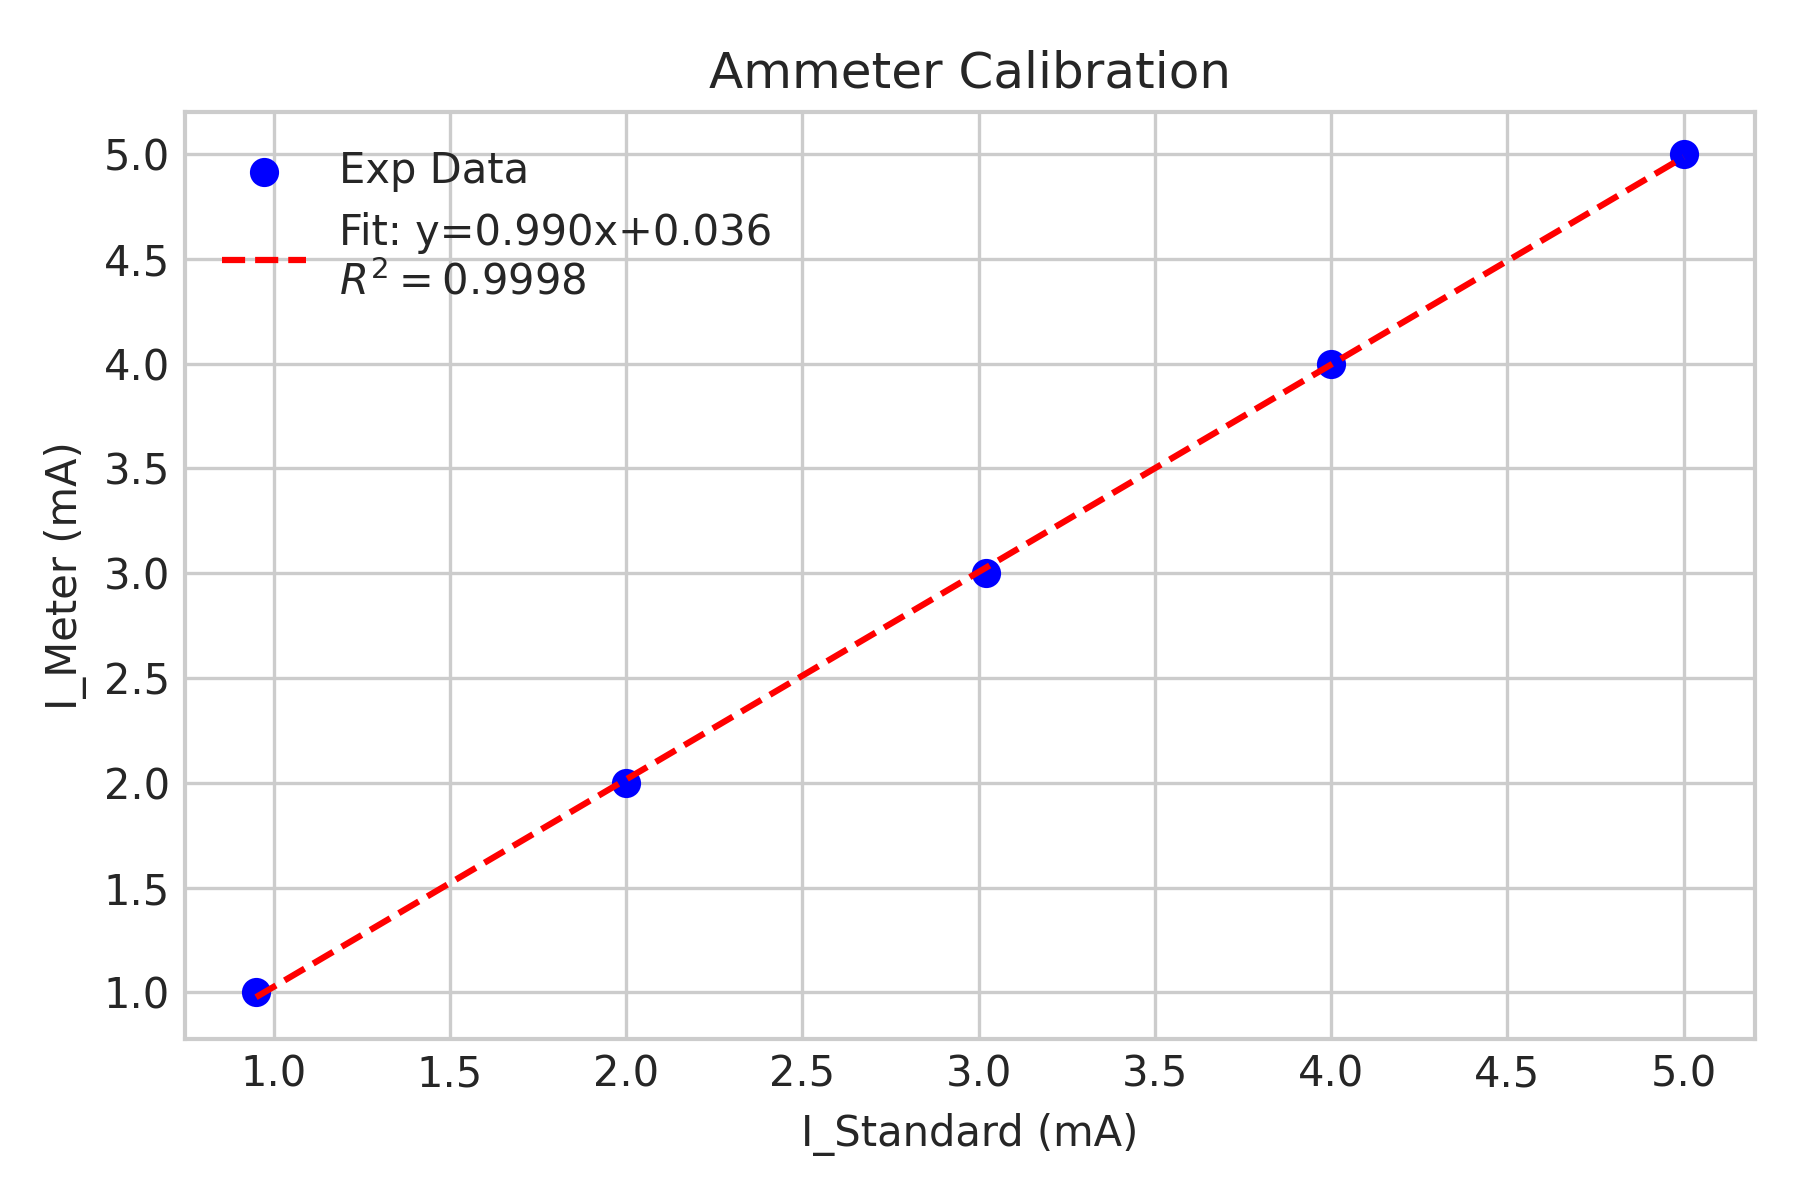
\includegraphics[width=\textwidth]{./figures/3/relaA.png}
            \caption{$I_G - I_B$ 校验曲线}
            \label{relaA}
        \end{subfigure}
        \hfill
        \begin{subfigure}[b]{0.48\textwidth}
            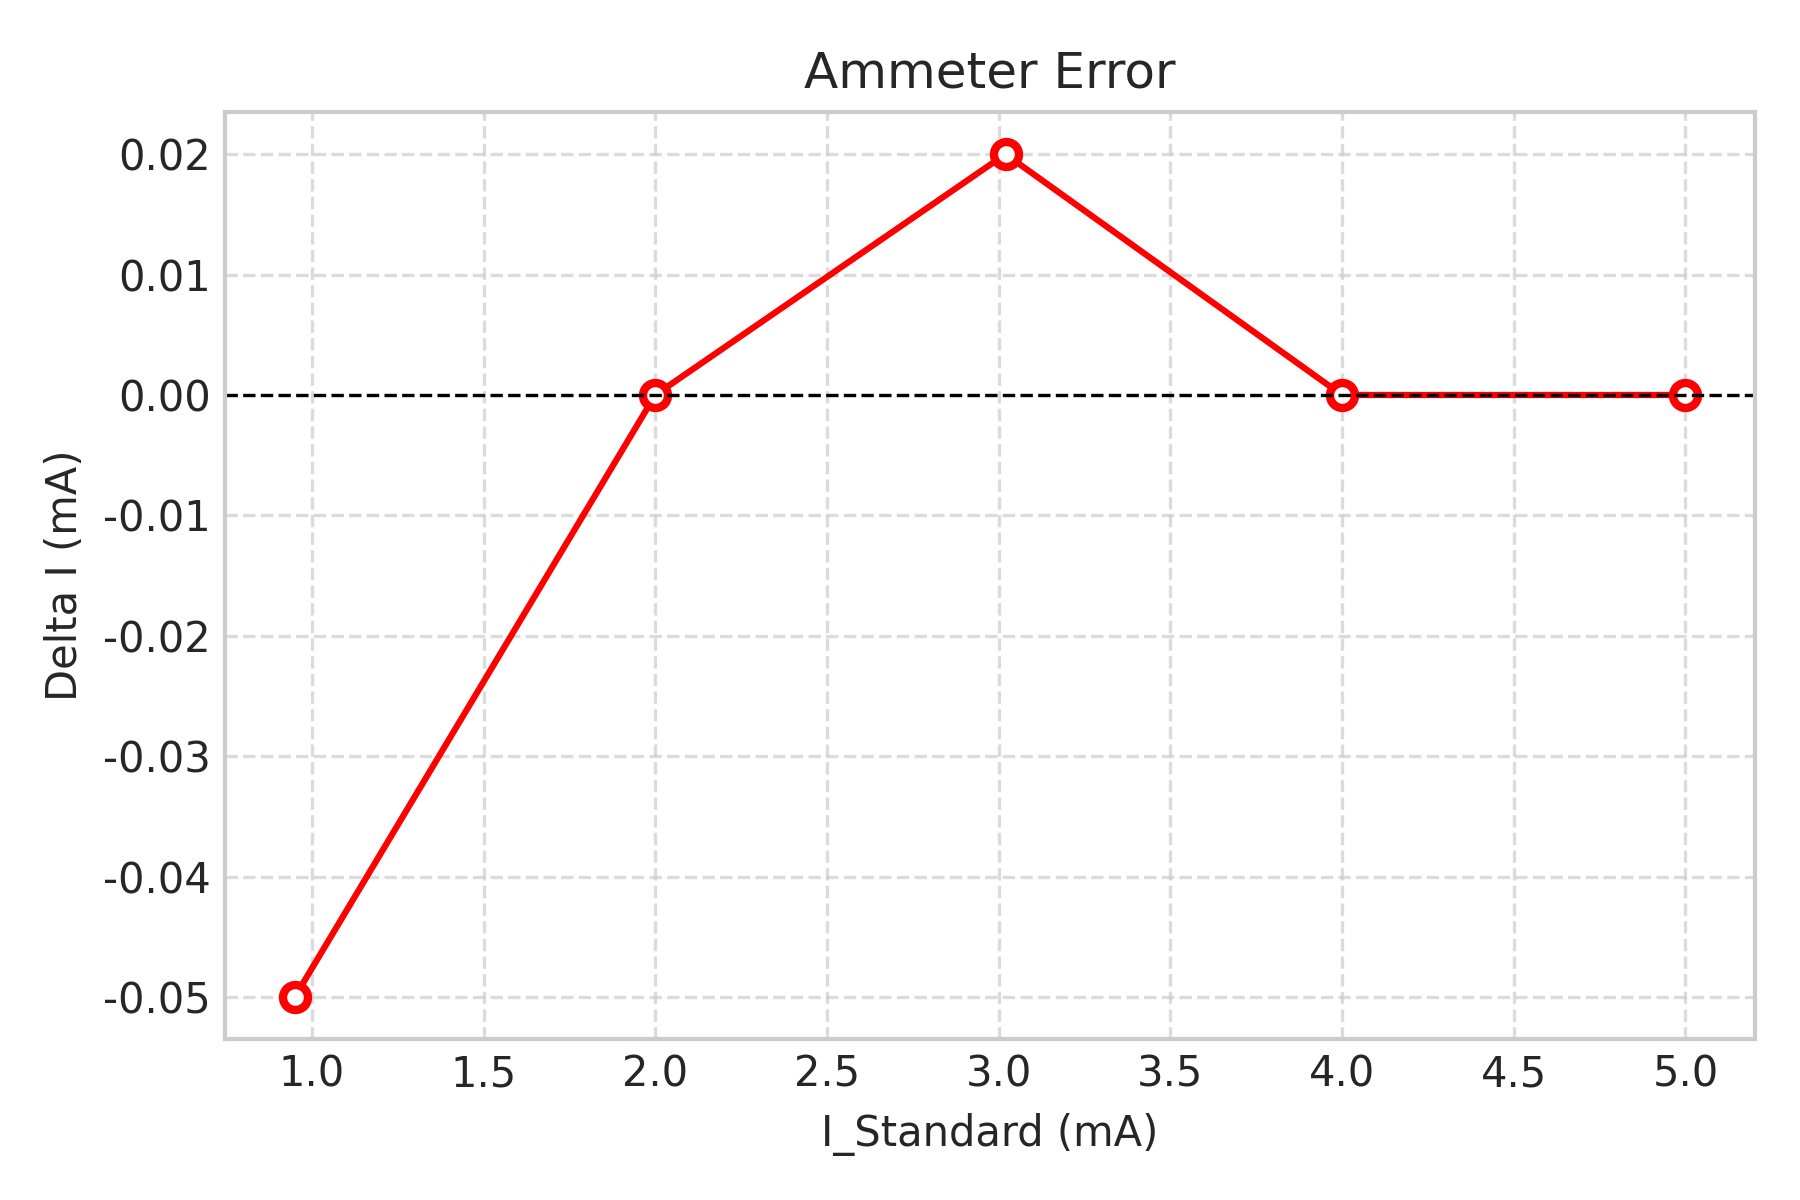
\includegraphics[width=\textwidth]{./figures/3/deltaA.png}
            \caption{$\Delta I - I_{\text{校准}}$ 误差分布曲线}
            \label{deltaA}
        \end{subfigure}
        \caption{改装电流表特性分析图}
        \label{fig:ampere_analysis}
    \end{figure}

    \subsubsection{电压表的设计、改装与校准}
    改装后的电压表量程为 $\SI{5}{V}$，分度值为 $\SI{0.1}{V}$。校准数据如 \cref{tableV} 所示。

    \begin{table}[H]
        \centering
        \caption{改装 $\SI{5}{V}$ 电压表校准数据记录}
        \begin{tabular}{C{0.1\textwidth} C{0.15\textwidth} C{0.15\textwidth} C{0.15\textwidth} C{0.15\textwidth} C{0.15\textwidth}}
            \toprule
            序号 & $V_{\text{G}} (\si{V})$ & $V_{\text{B}} (\si{V})$ & $\Delta V (\si{V})$ & $\varepsilon_r$ & $R_3 (\si{\ohm})$ \\
            \midrule
            1  & 1.00                    & 0.97                    & -0.03               & -3.1\%          & 956.0             \\
            2  & 2.00                    & 2.00                    & 0.00                & 0.0\%           & 956.0             \\
            3  & 3.00                    & 3.00                    & 0.00                & 0.0\%           & 956.0             \\
            4  & 4.00                    & 4.01                    & 0.01                & 0.2\%           & 956.0             \\
            5  & 5.00                    & 5.00                    & 0.00                & 0.0\%           & 956.0             \\
            \bottomrule
        \end{tabular}
        \label{tableV}
    \end{table}

    计算得最大绝对误差 $\Delta_{max} = |-0.03| = \SI{0.03}{V}$。
    其准确度判定指数为 $\left| \frac{\Delta_{max}}{0.1}\right| = \left| \frac{0.03}{0.1}\right| = 0.3$，故判定该改装电压表等级为 0.5 级。
    电压表校准特性曲线及误差分布图如 \cref{fig:volt_analysis} 所示。

    \begin{figure}[H]
        \centering
        \begin{subfigure}[b]{0.48\textwidth}
            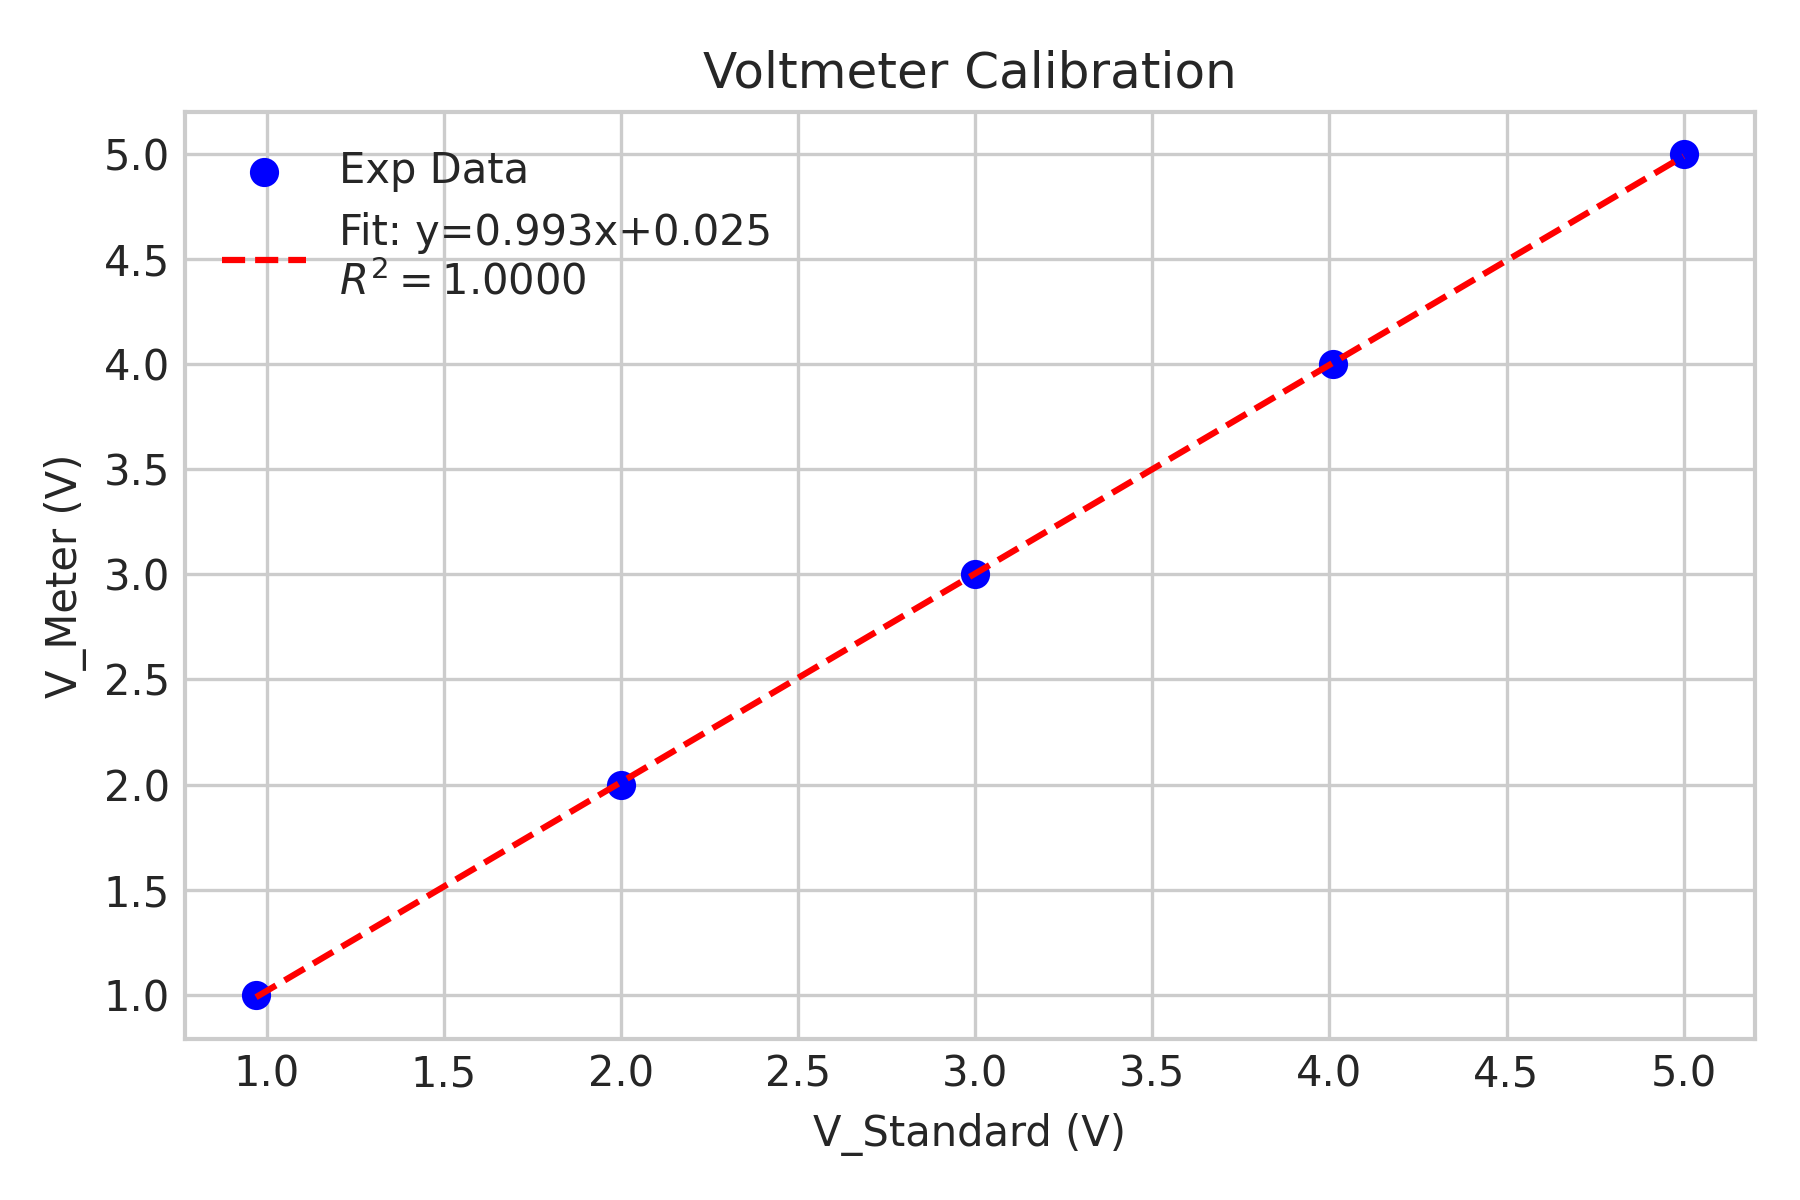
\includegraphics[width=\textwidth]{./figures/3/relaV.png}
            \caption{$V_G - V_B$ 校验曲线}
            \label{relaV}
        \end{subfigure}
        \hfill
        \begin{subfigure}[b]{0.48\textwidth}
            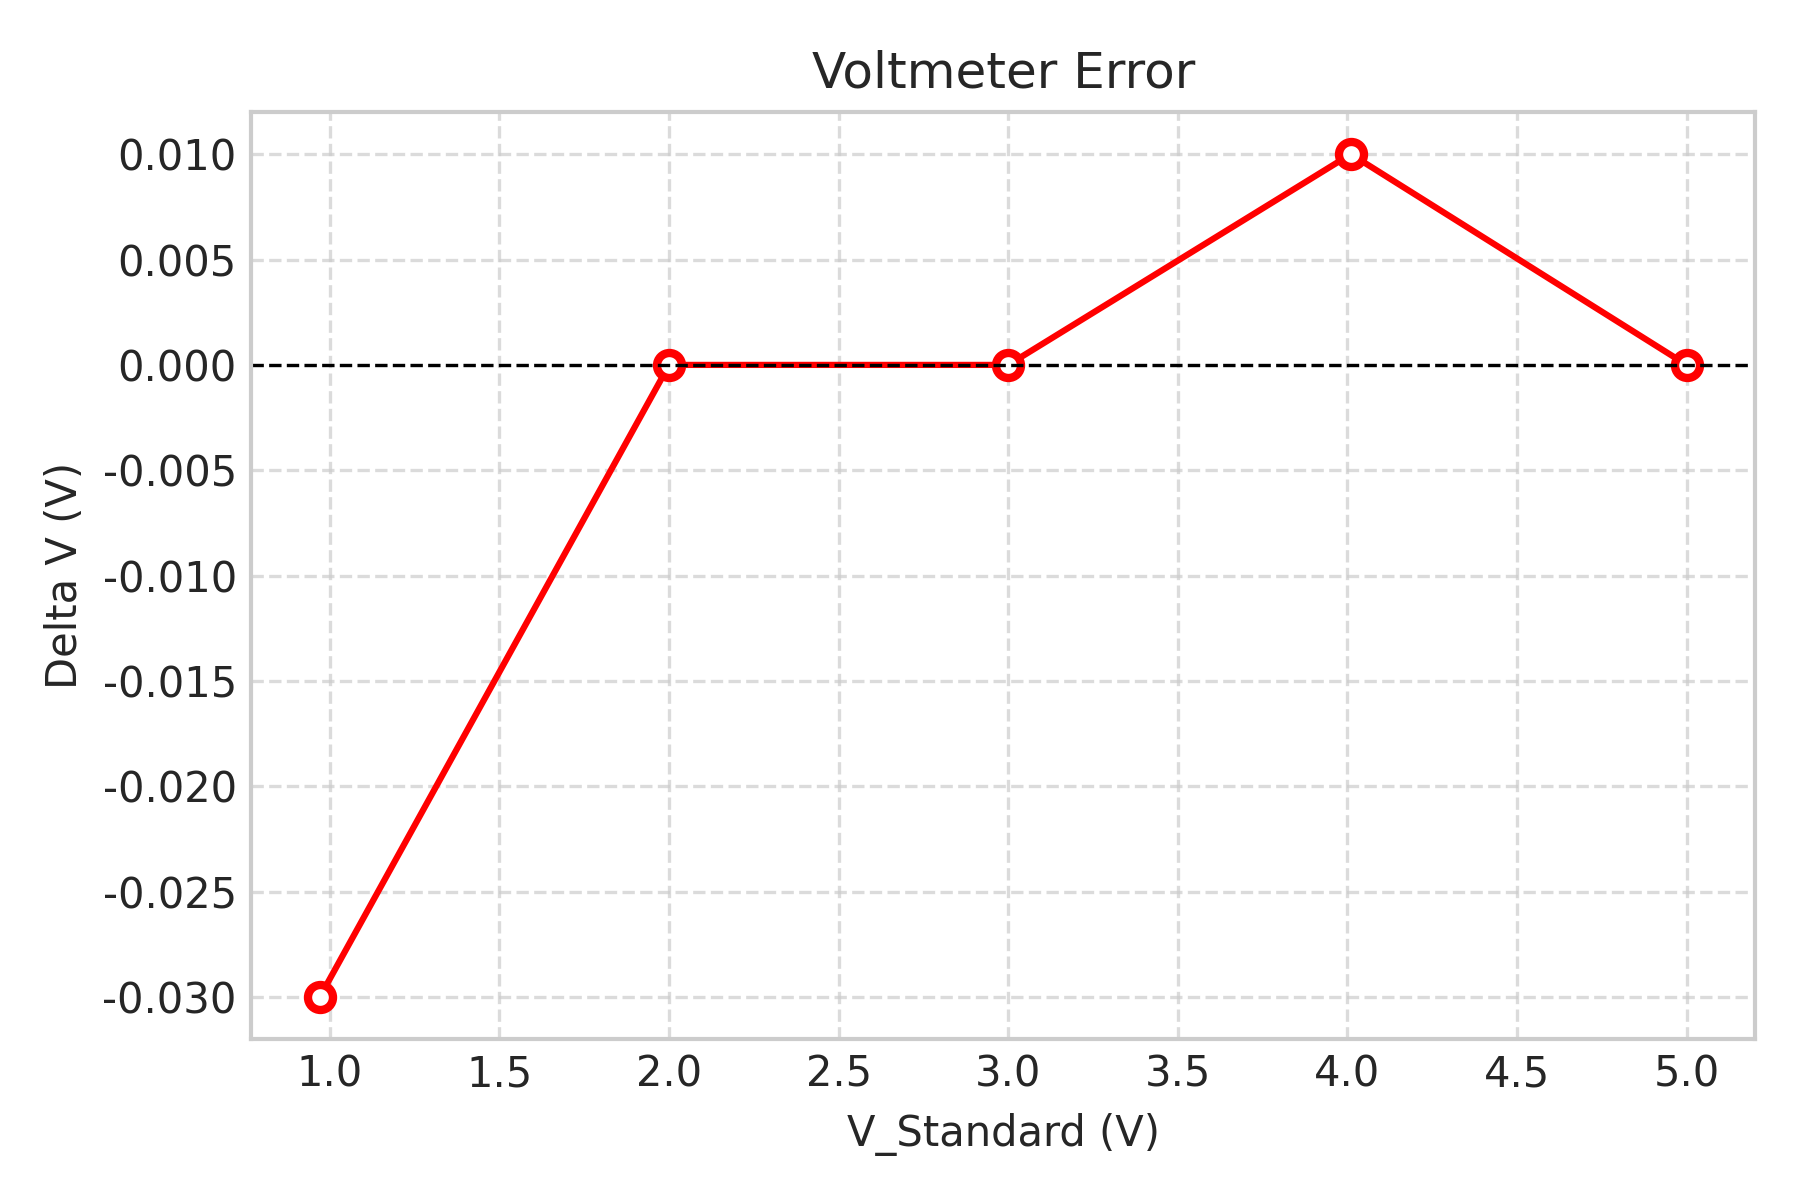
\includegraphics[width=\textwidth]{./figures/3/deltaV.png}
            \caption{$\Delta V - V_{\text{校准}}$ 误差分布曲线}
            \label{deltaV}
        \end{subfigure}
        \caption{改装电压表特性分析图}
        \label{fig:volt_analysis}
    \end{figure}

    \subsubsection{欧姆表的设计与特性分析}
    进行欧姆调零操作，调节电阻箱使表头指针指在满偏电流的一半处，初步测定中值电阻约为 $300 \si{\ohm}$。
    记录不同外接电阻 $R_x$ 下的电流 $I_x$ 测量数据如 \cref{tableOhm} 所示。

    \begin{table}[H]
        \centering
        \caption{改装欧姆表 $I_x - R_x$ 关系测量数据}
        \begin{tabular}{C{0.15\textwidth} C{0.25\textwidth} C{0.25\textwidth}}
            \toprule
            序号 & $R_x (\si{\ohm})$ & $I_x (\si{mA})$ \\
            \midrule
            1  & 100.0             & 0.721           \\
            2  & 200.0             & 0.600           \\
            3  & 300.0             & 0.449           \\
            4  & 400.0             & 0.410           \\
            5  & 500.0             & 0.390           \\
            6  & 600.0             & 0.265           \\
            7  & 700.0             & 0.249           \\
            8  & 800.0             & 0.235           \\
            9  & 900.0             & 0.222           \\
            10 & 1000.0            & 0.215           \\
            \bottomrule
        \end{tabular}
        \label{tableOhm}
    \end{table}

    分别绘制 $I_x - R_x$ 原始特性曲线（\cref{graphOhm}）以及线性化处理后的 $1/I_x - R_x$ 拟合曲线（\cref{ohmLinear}）。

    \begin{figure}[H]
        \centering
        \begin{subfigure}[b]{0.48\textwidth}
            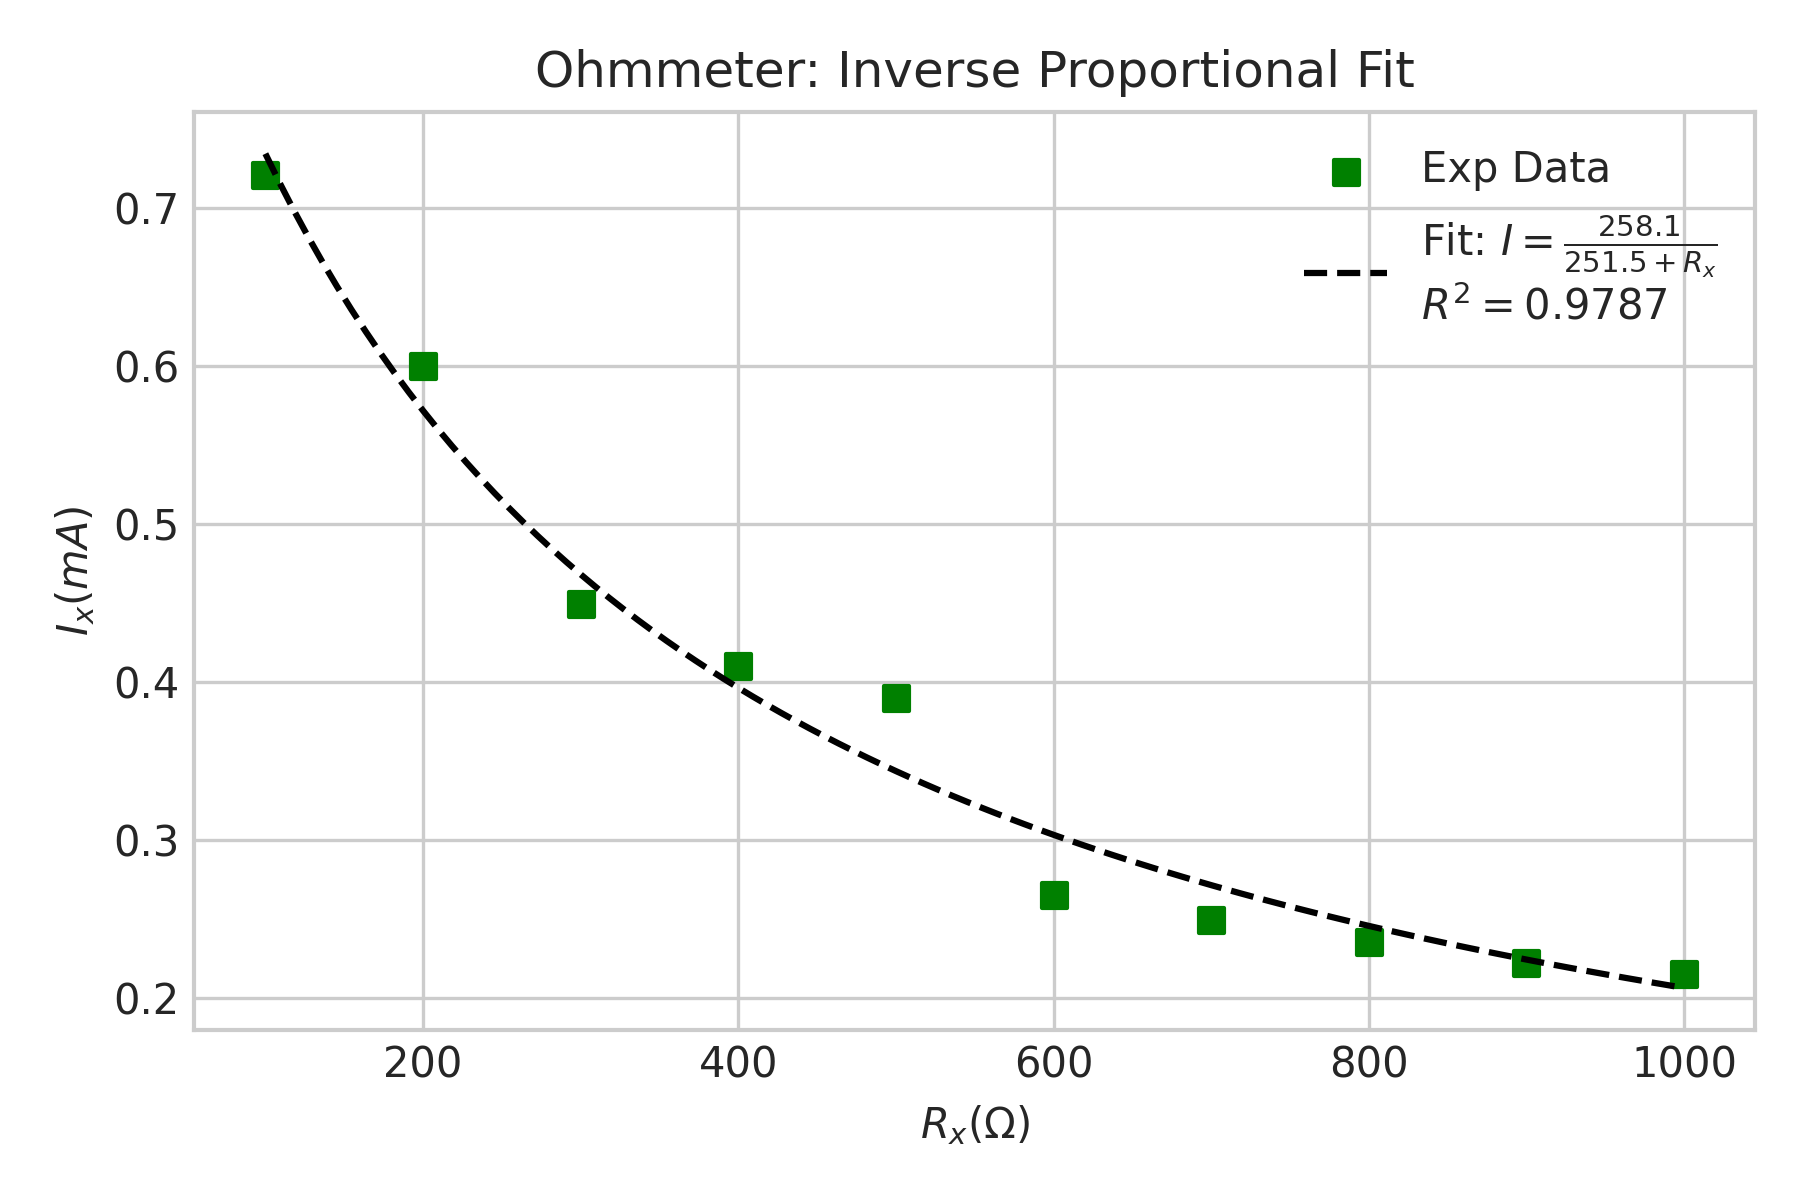
\includegraphics[width=\textwidth]{./figures/3/graphOhm.png}
            \caption{$I_x - R_x$ 反比例拟合}
            \label{graphOhm}
        \end{subfigure}
        \hfill
        \begin{subfigure}[b]{0.48\textwidth}
            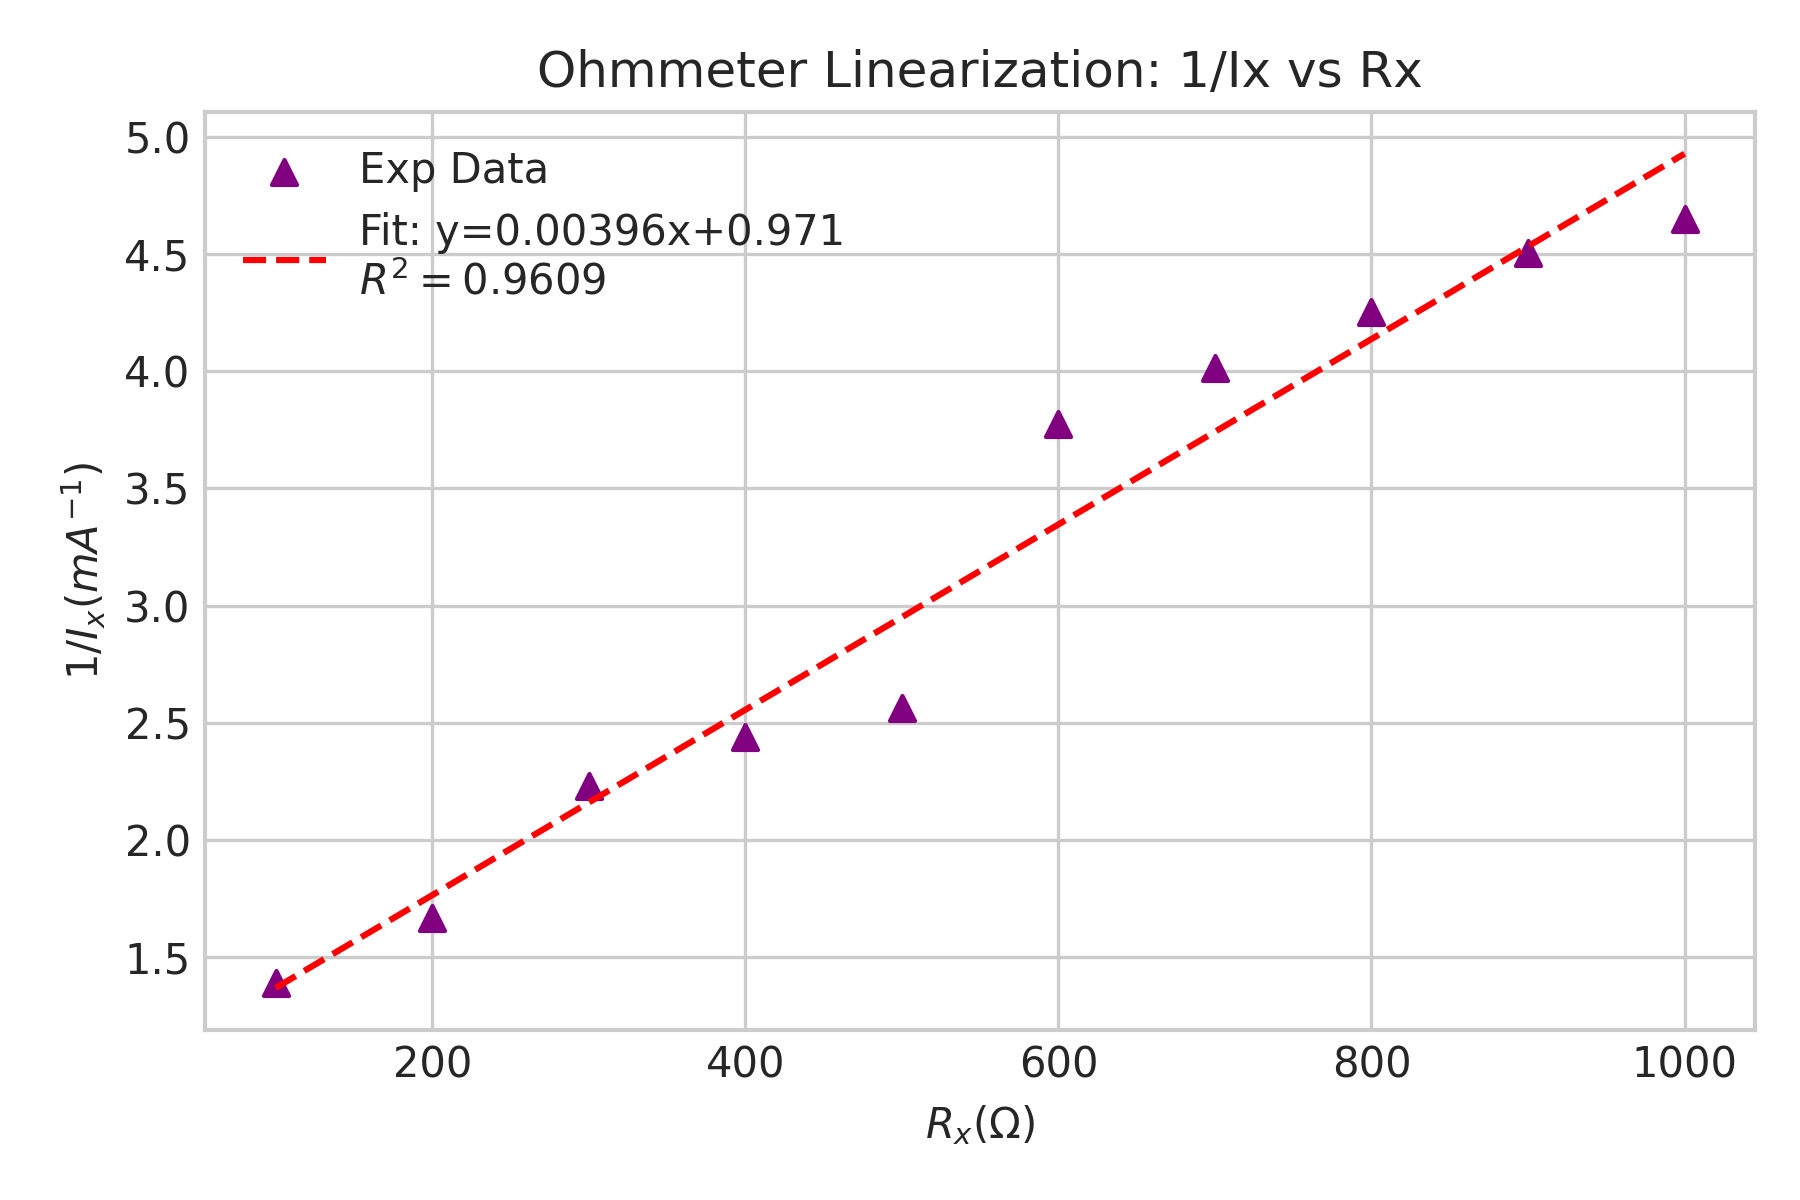
\includegraphics[width=\textwidth]{./figures/3/ohm_linear.png}
            \caption{$1/I_x - R_x$ 线性拟合}
            \label{ohmLinear}
        \end{subfigure}
        \caption{欧姆表改装实验数据分析}
    \end{figure}

    由 \cref{graphOhm} 可见，流经表头的电流 $I_x$ 与待测电阻 $R_x$ 呈非线性反比关系，验证了欧姆表刻度“左密右疏”的特点。
    为了验证欧姆闭合电路定律 $I_x = \frac{E}{R_{\text{中值}} + R_x}$，对数据进行线性化处理。由 \cref{ohmLinear} 可知，数据点呈现线性关系（$R^2 \approx 0.96$），符合理论情况。
    根据非线性拟合结果（见图 \ref{graphOhm}），该结果与理论模型基本符合。
    \subsection{误差分析（20分）}
    （运用测量误差、相对误差或不确定度等分析实验结果，写出完整的结果表达式，并分析误差原因。）

    本实验中，各测量点均只进行了一次测量，属于单次测量，故不计算 A 类不确定度。
    根据前述数据处理结果，改装电流表的最大绝对误差 $\Delta_{\text{max},A} = \SI{0.05}{mA}$，改装电压表的最大绝对误差 $\Delta_{\text{max},V} = \SI{0.03}{V}$。
    若按最大误差呈均匀分布估计，则改装表的 B 类不确定度分别为：
    \begin{equation}
        u_{b\_A} = \frac{\Delta_{\text{max},A}}{\sqrt{3}} = \frac{0.05}{\sqrt{3}} \approx \SI{0.029}{mA}
    \end{equation}
    \begin{equation}
        u_{b\_V} = \frac{\Delta_{\text{max},V}}{\sqrt{3}} = \frac{0.03}{\sqrt{3}} \approx \SI{0.017}{V}
    \end{equation}

    综合分析实验过程，本实验误差的主要来源可归纳为以下几点：

    \begin{enumerate}
        \item \textbf{仪器精度与灵敏度限制}：
              实验所用的微安表头、电阻箱以及作为标准的数字万用表均存在一定的精度限制。特别是在校准过程中发现，当调节电阻箱个位甚至十位数值时，模拟表头的指针位置几乎无肉眼可见的变化，这种灵敏度的局限性导致了校准电阻 $R_1, R_3$ 的设定值并非理论最优值，从而引入系统误差。

        \item \textbf{读数视差与人为误差}：
              由于改装表盘较小，且指针与刻度盘之间存在一定距离，读数时视线若未严格垂直于表盘，可能会产生视差。

        \item \textbf{接触电阻与线路影响}：
              实验主要在面包板上进行，导线连接处及元件管脚可能存在接触电阻。特别是在电流表改装和欧姆表设计中，线路和接触点的额外电阻会对电路分流、分压产生一定的影响。

        \item \textbf{仪器稳定性与随机干扰}：
              实验过程中观察到表头指针存在抖动现象，且单次测量无法通过统计平均来消除偶然误差，这也影响了最终数据的准确性。
    \end{enumerate}
    \subsection{实验探讨（10分）}
    （对实验内容、现象和过程的小结，不超过100字。）


    本次实验回顾了高中物理中关于万用表的实验，并以此为基础使我掌握了大学物理实验的规范和数据处理方法。
    在本次实验中，我不仅学会了面包板的使用，还掌握了用Python等现代化工具处理和分析数据。

    \section{思考题（10分）}
    （解答教材或讲义或老师布置的思考题，请先写题干，再作答。）

    \subsection{为什么不能用万用表欧姆挡直接测量电源内阻？}
    这个问题主要涉及测量原理冲突与仪器安全两个方面：
    \begin{enumerate}
        \item \textbf{有源网络与无源元件}：
              万用表欧姆挡的工作原理基于闭合电路欧姆定律，其前提是待测元件为“无源电阻”。测量时，仪表内部电池提供电压 $E_{\text{表}}$，通过测量电流 $I = \frac{E_{\text{表}}}{R_{\text{内}} + R_x}$ 来反推 $R_x$。
              若待测对象是一个有源网络，那么该电源的电动势 $E_x$ 会叠加在测量回路中，使得电路中的电流变为 $I' = \frac{E_{\text{表}} \pm E_x}{R_{\text{内}} + r}$。此时，仪表既定的电阻-电流对应关系失效，导致测量结果完全错误。

        \item \textbf{仪器安全风险}：
              欧姆挡的内阻通常较小。若直接连接电压较高的外部电源，相当于将电源短路或加载在低阻负载上，回路中可能产生极大电流，极易烧毁万用表的表头线圈、分流电阻或熔断保险丝。
    \end{enumerate}

    \subsection{为什么不能用欧姆表直接测量另一个微安表头的内阻？}
    直接测量存在极大的损坏风险，且测量精度难以保证：
    \begin{enumerate}
        \item \textbf{过载损坏风险}：
              待测微安表头极其灵敏，满偏电流 $I_g$ 很小。而普通欧姆表在测量低电阻时，输出的短路电流往往达到毫安甚至几十毫安级别，远超表头的承受极限。直接测量极易导致指针打弯，甚至烧毁动圈。

        \item \textbf{测量精度问题}：
              表头内阻通常在几百欧姆至几千欧姆之间。若使用欧姆表的大倍率挡，读数偏差大；若使用小倍率挡，虽然读数可能落在刻度范围内，但又面临上述的过载风险。

        \item \textbf{改进测量方案}：
              若必须使用欧姆表测量，建议采用“串联限流法”。即在表头电路中串联一个已知阻值的电阻箱 $R_{\text{box}}$来保护表头，调节电阻箱使总阻值落在欧姆表中心刻度附近。测得总阻值 $R_{\text{total}}$ 后，利用 $R_g = R_{\text{total}} - R_{\text{box}}$ 间接求得内阻。
    \end{enumerate}

    \subsection{为什么 $I_x$ 与 $R_x$ 为非线性关系？}
    这由闭合电路欧姆定律所决定。
    设欧姆表内部电源电动势为 $E$，总内阻为 $R_{\text{中值}}$。当外接电阻 $R_x$ 时，流过表头的电流 $I_x$ 为：
    \begin{equation}
        I_x = \frac{E}{R_{\text{中值}} + R_x}
    \end{equation}
    对此式进行分析可知：
    \begin{enumerate}
        \item \textbf{数学关系}：$I_x$ 是关于 $R_x$ 的反比例函数，而非线性函数 $I_x = k \cdot R_x + b$。
        \item \textbf{物理意义}：随着 $R_x$ 线性增加，分母变大，电流 $I_x$ 非线性减小。
        \item \textbf{图表验证}：实验数据的 $I_x - R_x$ 拟合曲线呈现出明显的下凹双曲线特征，且刻度盘上体现为“左密右疏、反向刻度”的分布，这均是该非线性关系的直观体现。
    \end{enumerate}
\end{fullreportonly}
\insertnotes
\end{document}